% Konferans bildirisi (IEEE konferans sablonu, A4, iki sutun, en fazla 6 sayfa, cift kor).
% Derleme: cd bildiri && latexmk -pdf bildiri.tex
% Sekiller ve tablo satirlari: python3 scripts/bildiri_figures.py
\documentclass[conference,a4paper]{IEEEtran}
\usepackage[T1]{fontenc}
\usepackage[utf8]{inputenc}
\usepackage[english,turkish,shorthands=off]{babel}
\usepackage{amsmath,amssymb}
\usepackage{graphicx}
\usepackage{booktabs}
\usepackage{cite}
\usepackage{url}
\newcommand{\tri}{\operatorname{tri}}
\renewcommand{\IEEEkeywordsname}{Anahtar Kelimeler}
\makeatletter\newcommand{\satirlar}[1]{\@@input #1 }\makeatother

\begin{document}

\title{Sürekli Öğrenmede Plastisite Kaybı ve Sınırlı Ağırlık Yeniden Parametrizasyonları:
Sinüs, Tanh ve Üçgen Dalga Haritaları Üzerine Bir Ön Çalışma\\[4pt]
{\large Loss of Plasticity in Continual Learning and Bounded Weight Reparameterizations:
A Preliminary Study of Sine, Tanh and Triangle-Wave Maps}}

\author{\IEEEauthorblockN{Çift kör değerlendirme için yazar bilgileri çıkarılmıştır}}

\maketitle

\begin{abstract}
Uzun bir görev dizisi üzerinde eğitilen yapay sinir ağları yeni görevleri öğrenme yeteneğini zamanla yitirir;
bu olgu plastisite kaybı olarak adlandırılır. Bilinen nedenlerden biri ağırlık büyüklüğünün artmasıdır ve
ağırlıkları sabit bir aralıkta tutmak etkili bir çaredir. Bu ön çalışmada sınırlılığın tek başına yeterli olup
olmadığı deneysel olarak incelenmiştir. Her ağırlık $W=A\,f(\Theta/A)$ biçiminde yazılmış; düzgün ve periyodik
(sinüs), düzgün ve periyodik olmayan (tanh) ve parçalı doğrusal periyodik (üçgen dalga) haritalar, standart ağ ve
ağırlık kırpma ile karşılaştırılmıştır. Çevrim içi Permütasyonlu MNIST üzerinde 200 görevlik akışta ve en çok on
eşleştirilmiş tohumla yapılan deneylerde düzgün haritalar standart ağdan biraz iyi sonuç vermiş, ancak
plastisiteyi koruyamamıştır (koruma oranı 0,93; standart ağda 0,91). Bu modellerde ağırlıklar haritanın
türevinin sıfıra yaklaştığı sınıra doğru kaymış, ortalama adım çarpanı sinüste 0,85'ten 0,56'ya, tanh'ta
0,74'ten 0,47'ye düşmüştür. Türevinin büyüklüğü köşe noktaları dışında bir olan üçgen dalga ise kayıp
göstermemiş (koruma oranı 1,02) ve ağırlık kırpmadan ayırt edilememiştir; onu geçtiği de gözlenmemiştir.
Bulgular tek bir veri kümesi, küçük bir ağ ve kısa bir akışla sınırlıdır.
\end{abstract}

\begin{IEEEkeywords}
sürekli öğrenme, plastisite kaybı, ağırlık yeniden parametrizasyonu, ağırlık kırpma, üçgen dalga
\end{IEEEkeywords}

\begin{otherlanguage}{english}
\renewcommand{\abstractname}{Abstract}
\renewcommand{\IEEEkeywordsname}{Keywords}
\begin{abstract}
Neural networks trained on a long sequence of tasks gradually lose the ability to learn new ones, a phenomenon
known as loss of plasticity. Growth of the weight magnitude is one known cause, and keeping the weights inside a
fixed interval is an effective remedy. This preliminary study examines empirically whether boundedness alone is
sufficient. Each weight is written as $W=A\,f(\Theta/A)$, and a smooth periodic map (sine), a smooth non-periodic
map (tanh) and a piecewise-linear periodic map (triangle wave) are compared with the standard network and with
weight clipping. On Online Permuted MNIST with a 200-task stream and up to ten paired seeds, the smooth maps are
slightly better than the standard network but do not preserve plasticity (retention ratio 0.93 versus 0.91).
Their weights drift towards the bound, where the derivative of the map approaches zero, and the mean step
multiplier falls from 0.85 to 0.56 for sine and from 0.74 to 0.47 for tanh. The triangle wave, whose derivative
has unit magnitude away from its corner points, shows no loss (retention ratio 1.02) and could not be
distinguished from weight clipping; it was not observed to improve on it. The findings are limited to one
dataset, a small network and a short stream.
\end{abstract}
\begin{IEEEkeywords}
continual learning, loss of plasticity, weight reparameterization, weight clipping, triangle wave
\end{IEEEkeywords}
\end{otherlanguage}

% ----------------------------------------------------------------------------------------------------
\section{Giriş}

Sürekli öğrenmede bir ağ, sonu olmayan bir görev akışı üzerinde eğitilir ve bininci görevi ilk görev kadar iyi
öğrenmesi beklenir. Geri yayılımla eğitilen standart ağlar bu beklentiyi karşılamaz: yeterince görevden sonra
yeni görevleri, sıfırdan başlatılmış bir ağa göre daha yavaş ve daha düşük doğrulukla öğrenirler
\cite{ash2020warm,lyle2023understanding,dohare2024loss}. Bu olgu \emph{plastisite kaybı}
olarak adlandırılır ve eski görevlerle ilgili olan yıkıcı unutmadan farklıdır; yeni bilgi edinme yeteneğiyle
ilgilidir.

Olgu için birden çok mekanizma öne sürülmüştür: ölü ya da uyuyan birimler \cite{sokar2023dormant,abbas2023loss},
temsil kertesinin düşmesi \cite{lyle2022understanding,dohare2024loss} ve ağırlık büyüklüğünün artması
\cite{dohare2024loss,elsayed2024weight,lyle2024normalization}. Bu mekanizmalar birlikte etki eder
\cite{lyle2024disentangling}. Ağırlık büyüklüğünü hedefleyen çareler arasında en yalın olanı \emph{ağırlık
kırpmadır} (weight clipping) \cite{elsayed2024weight}: her güncellemeden sonra her ağırlık, genişliği katmanın
başlatma ölçeği $b$ ile belirlenen $[-\kappa b,\kappa b]$ aralığına geri izdüşürülür.

Kırpma, eniyileyici adımından \emph{sonra} uygulanan bir işlemdir. Aynı kısıt, her ağırlığı serbest bir
parametrenin sınırlı bir fonksiyonu olarak yazarak \emph{yapısal} biçimde de sağlanabilir:
\begin{equation}
  W = A\, f(\Theta/A), \qquad f:\mathbb{R}\to[-1,1]. \label{eq:reparam}
\end{equation}
Böylece $|W|\le A$ koşulu $\Theta$'nın her değeri için kendiliğinden sağlanır ve izdüşüm adımına gerek kalmaz.
Bu çalışmanın başlangıç varsayımı, $f=\sin$ seçiminin ağırlıkları sınırlı tuttuğu için plastisiteyi koruyacağı
yönündeydi. Deneyler bu varsayımı desteklememiştir. Bu bildiride varsayımın neden tutmadığı ve hangi haritanın
işe yaradığı, kısa bir akış üzerindeki ön sonuçlarla raporlanmaktadır.

Katkılar şunlardır: (i)~Düzgün sınırlı haritaların (sinüs, tanh) 200 görevlik akışta plastisiteyi korumadığı,
on eşleştirilmiş tohumla gösterilmiştir. (ii)~Bunun, sınırda haritanın türevinin küçülmesinden kaynaklanan
adım sönümlemesiyle uyumlu olduğu ölçümlerle ortaya konmuştur. (iii)~Türevi sıfıra yaklaşmayan periyodik bir
haritanın (üçgen dalga) kayıp göstermediği ve ağırlık kırpma ile aynı sonucu verdiği bulunmuştur. Çalışma ağırlık
kırpmayı geçen bir yöntem önermemektedir; katkı, sınırlı bir parametrizasyonun \emph{hangi özelliğinin} önemli
olduğuna ilişkin deneysel bir gözlemdir.

% ----------------------------------------------------------------------------------------------------
\section{İlgili Çalışmalar}

Önceden eğitilmiş ağların sıfırdan başlatılanlara göre daha kötü genellediği \cite{ash2020warm} ve bu etkinin uzun
görev dizilerinde biriktiği \cite{dohare2024loss} gösterilmiştir. Ağırlık büyüklüğünü
denetleyen yöntemler arasında başlangıç parametrelerine doğru düzenlileştirme \cite{kumar2023maintaining},
normalizasyon sonrası norm izdüşümü \cite{lyle2024normalization} ve ağırlık kırpma \cite{elsayed2024weight}
sayılabilir. Lyle vd. \cite{lyle2024disentangling} mekanizmaların büyük ölçüde bağımsız olduğunu ve katman
normalizasyonu ile ağırlık azaltımının birlikte kullanılmasının birkaçını birden giderdiğini bildirmiştir.

Periyodik fonksiyonlar sürekli öğrenmede \emph{aktivasyon} olarak incelenmiştir: her katmanda sinüs ve kosinüsün
birlikte kullanılması ağları eğitilebilir tutmuş \cite{lewandowski2025fourier}, plastisite ile aktivasyonun
türevinin sıfırdan uzak kalması arasında ilişki kurulmuştur \cite{lillo2026activation}. Sinüs aktivasyonlu,
ağırlıkları sınırsız klasik bir ağın ise plastisite kaybettiği bildirilmiştir \cite{chen2026intrinsic}. Bu
çalışmalar birimin hesapladığı fonksiyonu değiştirir. Burada periyodik harita \emph{ağırlıklara} uygulanır: ağ,
$W$ açısından standart bir ReLU ağı olarak kalır; yalnızca eniyileyicinin hareket ettiği koordinatlar değişir.
Ağırlıkları başka parametrelerin fonksiyonu olarak yazmak, fonksiyon sınıfını değiştirmeden eniyileme
geometrisini değiştirir \cite{salimans2016weight}. Üçgen dalga, gradyan büyüklüğü sabit bir harita olarak yeni
değildir; bir sinirsel şekil parametrizasyonunda sinüse tercih edilmiştir \cite{dai2025shaping}. Sınırlı
periyodik yeniden parametrizasyonu ağ ağırlıklarına plastisite kaybı bağlamında uygulayan bir çalışmaya
yaptığımız taramada rastlanmamıştır; tarama kapsamlı bir sistematik derleme değildir.

% ----------------------------------------------------------------------------------------------------
\section{Yöntem}

\subsection{Sınırlı yeniden parametrizasyon}

Giriş sayısı $n$ olan tam bağlı bir katmanın ağırlıkları, Kaiming sınırı $b=\sqrt{6/n}$ ile $[-b,b]$ aralığından
düzgün dağılımla başlatılır \cite{he2015delving}. Genlik $A=\gamma b$ ($\gamma\ge1$) olarak sabitlenir ve her
ağırlık ile her sapma terimi \eqref{eq:reparam} ile serbest bir $\Theta$ parametresine bağlanır. Üç harita
incelenmiştir (Şekil~\ref{fig:haritalar}):
\begin{align}
  \text{sinüs:}\quad & f(x)=\sin x, & f'(x)&=\cos x, \nonumber\\
  \text{tanh:}\quad & f(x)=\tanh x, & f'(x)&=1-\tanh^2 x, \nonumber\\
  \text{üçgen:}\quad & f(x)=\tri(x), & |f'(x)|&=1 .
\end{align}
Burada $\tri(x)=\tfrac{2}{\pi}\arcsin(\sin(\tfrac{\pi}{2}x))$ periyodu 4 olan üçgen dalgadır; $[-1,1]$
aralığında birim fonksiyona eşittir ve $\pm1$ noktalarında yansır. Türevi yükselen kollarda $+1$, inen kollarda
$-1$ olup köşe noktalarında tanımlı değildir; uygulamada bu noktalarda sağdan türev kullanılmıştır. Bütün
modeller aynı etkin ağırlıklardan başlar: $W_0$ bir kez çekilir ve $\Theta_0=A f^{-1}(W_0/A)$ alınır.

\begin{figure}[t]
  \centering
  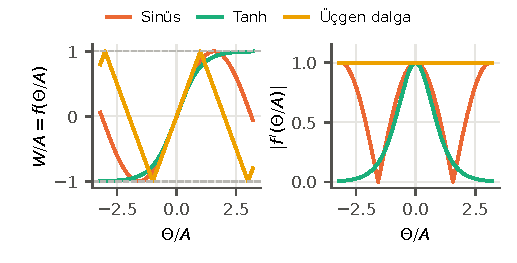
\includegraphics[width=\linewidth]{figures/sekil_haritalar.pdf}
  \caption{Üç sınırlı harita (solda) ve türevlerinin büyüklüğü (sağda). Düzgün haritaların türevi sınırda sıfıra
  gider; üçgen dalganınki köşe noktaları dışında birdir.}
  \label{fig:haritalar}
\end{figure}

\subsection{Jacobian sönümlemesi}

$g=\partial L/\partial W$ olsun. $\Theta$ üzerinde $\eta$ öğrenme oranıyla atılan bir stokastik gradyan adımı,
etkin ağırlığı birinci mertebeden
\begin{equation}
  \Delta W \approx f'(\Theta/A)\,\Delta\Theta = -\eta\, f'(\Theta/A)^2\, g \label{eq:sonum}
\end{equation}
kadar değiştirir. $f'^2\in[0,1]$ çarpanı, her parametre için ayrı bir öğrenme oranı çarpanıdır; bu çalışmada
\emph{adım çarpanı} olarak adlandırılmıştır. Sinüs haritasında $\cos^2(\Theta/A)=1-(W/A)^2$ değerini alır: ağırlık
sınıra yaklaştıkça adımı küçülür.

Türevlenebilir ve sınırına ulaşan bir $f$ için, sınıra ulaşılan nokta bir iç uç nokta olduğundan türev orada
sıfırdır. Dolayısıyla bir harita aynı anda düzgün, sınırına ulaşan ve türevi sıfırdan uzak olamaz. Düzgün bir
sınırlı harita ya sınırına ulaşır (sinüs) ve adım çarpanı sonlu bir $\Theta$ değerinde sıfırlanır, ya da sınıra
yalnızca asimptotik olarak yaklaşır (tanh) ve çarpan $|\Theta|$ büyüdükçe küçülmeyi sürdürür. İki durumda da
verinin sınıra ittiği bir ağırlık tam oraya vardığında yavaşlar ve geri dönüşü de aynı küçük adımlarla olur.
Düzgünlükten vazgeçmek bu ödünleşimi ortadan kaldırır: üçgen dalga sınırlıdır ve köşeler dışında $|f'|=1$'dir.

\subsection{Yansıma ve izdüşüm}\label{sec:yansima}

Üçgen dalgada \eqref{eq:sonum} aralığın içinde tam olarak $\Delta W=-\eta g$ verir. Ağırlığı $A+\delta$
değerine taşıyacak bir adım ($0<\delta<2A$) onu $A-\delta$ değerinde bırakır: ağırlık sınırda \emph{yansır}.
Ağırlık kırpma aynı adımı $A$ değerine eşler: ağırlık \emph{izdüşürülür}. Ortak bir başlangıç noktasından atılan
tek adımın ardından iki sonuç arasındaki fark en çok $\delta\le\eta|g|$ kadardır ve iki yöntem de gradyanı
ölçeklemez. Adımlar aralığın genişliğine göre küçük olduğunda, $\kappa=\gamma$ seçilmiş bir kırpma ile üçgen
dalganın $W$ uzayında birbirine yakın yörüngeler izlemesi beklenir.

% ----------------------------------------------------------------------------------------------------
\section{Deney Düzeni}

\textbf{Akış.} Çevrim içi Permütasyonlu MNIST \cite{goodfellow2013empirical,zenke2017continual,dohare2024loss}
kullanılmıştır: her görev, MNIST \cite{lecun1998gradient} görüntülerinin piksellerine yeni bir rastgele
permütasyon uygular. Akış 200 görevden oluşur; her görevde eğitim kümesinden rastgele seçilen 5.000 görüntü birer
birer (yığın boyutu bir) ve bir kez gösterilir. Görev sınırı ya da görev kimliği ağa verilmez. Bir koşu
$10^6$ güncellemeden oluşur.

\textbf{Ağ ve eniyileyici.} Her biri 100 birimli üç gizli katmanı olan ReLU çok katmanlı algılayıcı, yalın
stokastik gradyan inişi ile eğitilmiştir.

\textbf{Modeller.} (i)~Standart ağ; (ii--iv)~bütün ağırlık ve sapma terimlerinin sinüs, tanh ve üçgen dalga
ile yeniden parametrizasyonu; (v)~ağırlık kırpma \cite{elsayed2024weight}.

\textbf{Hiperparametreler.} Bütün değerler, değerlendirme akışlarıyla permütasyon paylaşmayan 100 görevlik ayrı
geliştirme akışlarında seçilmiş ve değerlendirme sırasında değiştirilmemiştir. Seçilen değerler: bütün modeller
için öğrenme oranı 0,003; sinüs ve tanh için $\gamma=1{,}5$; üçgen dalga için $\gamma=1$; kırpma için
$\kappa=1$.

\textbf{Ölçütler.} Performans ölçütü \emph{çevrim içi doğruluktur}: her görüntünün, o görüntüyle güncelleme
yapılmadan önce doğru sınıflandırılma oranı. \emph{AUC}, bütün görevler üzerindeki ortalama çevrim içi
doğruluktur. \emph{İlk} ve \emph{son pencere}, ilk ve son 20 görevin ortalamasıdır; \emph{koruma oranı} son
pencerenin ilk pencereye bölümüdür. \emph{Taze model farkı}, son görevde sıfırdan başlatılan bir ağın çevrim içi
doğruluğundan sürekli eğitilen ağınkinin çıkarılmasıyla bulunur; pozitif değer, sürekli eğitilen ağın başka hiçbir
görev görmemiş bir ağdan kötü olduğunu gösterir. Mekanizma ölçütleri olarak ortalama adım çarpanı
$\langle f'^2\rangle$, doymuş parametre oranı ($|f'|<0{,}1$), ortalama ağırlık büyüklüğü, gerçekleşen ağırlık
adımının normu ve son gizli katman temsilinin etkin kertesi \cite{roy2007effective} kaydedilmiştir.

\textbf{Tohumlar ve istatistik.} Standart ağ ve üç harita için on, ağırlık kırpma için beş tohum
çalıştırılmıştır. Bir tohum hem başlatmayı hem permütasyon dizisini belirler; modeller özdeş akışlarda
karşılaştırıldığından bütün farklar eşleştirilmiştir. Ortalamalar tohumlar üzerinden \%95 $t$-aralığıyla,
farklar eşleştirilmiş $t$-testiyle verilmiştir. Üçgen dalga ile ağırlık kırpma karşılaştırmasında anlamlı fark
bulunmaması eşitliğin kanıtı olmadığından, 0,005 eşdeğerlik sınırıyla iki tek yönlü test (TOST)
\cite{schuirmann1987comparison} uygulanmıştır.

% ----------------------------------------------------------------------------------------------------
\section{Bulgular}

\subsection{Performans}

\begin{figure}[t]
  \centering
  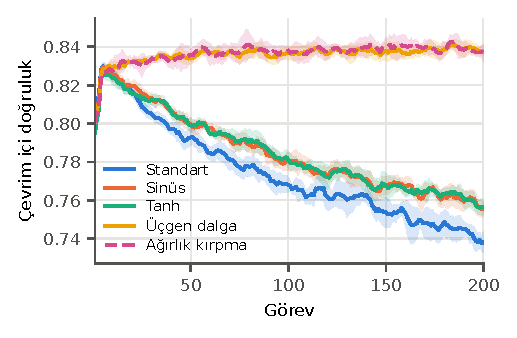
\includegraphics[width=\linewidth]{figures/sekil_dogruluk.pdf}
  \caption{200 görevlik akışta çevrim içi doğruluk (tohumlar üzerinden ortalama ve \%95 aralığı; beş görevlik
  kayan ortalama). Üçgen dalga ile ağırlık kırpma eğrileri üst üste binmektedir.}
  \label{fig:dogruluk}
\end{figure}

\begin{table}[t]
  \centering
  \caption{200 görevlik akışta sonuçlar (ortalama $\pm$ \%95 aralığı; $n$: tohum sayısı).}
  \label{tab:sonuclar}
  \setlength{\tabcolsep}{2.5pt}\footnotesize
  \resizebox{\linewidth}{!}{%
  \begin{tabular}{@{}lccccc@{}}
    \toprule
    Model & $n$ & AUC & Son pencere & Koruma oranı & Taze model farkı\\
    \midrule
    \satirlar{tablo_sonuclar.tex}
    \bottomrule
  \end{tabular}}
\end{table}

Şekil~\ref{fig:dogruluk} ve Tablo~\ref{tab:sonuclar} sonuçları özetlemektedir. Standart ağın çevrim içi doğruluğu
akış boyunca düşer: son pencere ilk pencerenin 0,906 katıdır ve son görevde sıfırdan başlatılan bir ağ, sürekli
eğitilen ağdan 0,021 daha yüksek doğruluk elde eder.

Sinüs ve tanh modelleri standart ağdan biraz iyidir: AUC farkı sırasıyla $+0{,}0110$ (\%95 aralığı
$[+0{,}0100;+0{,}0120]$) ve $+0{,}0109$ ($[+0{,}0095;+0{,}0123]$) olup on tohumun onunda da pozitiftir. Bununla
birlikte iki model de plastisite kaybeder: koruma oranları 0,926 ve 0,931'dir ve eğrileri standart ağınkine
koşut biçimde düşer. Sinüs ile tanh arasında AUC farkı bulunmamıştır ($+0{,}0001$, $p=0{,}87$).

Üçgen dalgada düşüş görülmez. Koruma oranı 1,017'dir; yani son 20 görevdeki doğruluk ilk 20 görevdekinden biraz
yüksektir. Standart ağa göre AUC farkı $+0{,}0616$ ($[+0{,}0595;+0{,}0636]$), sinüse göre $+0{,}0506$
($[+0{,}0486;+0{,}0525]$) olup iki karşılaştırmada da on tohumun onunda pozitiftir. Son görevde sürekli eğitilen
üçgen dalga ağı, sıfırdan başlatılan ağdan 0,080 daha iyidir; bu, önceki görevlerden olumlu aktarım olduğuna
işaret eder.

Üçgen dalga ile ağırlık kırpma arasındaki farklar, beş ortak tohumda, AUC için $+0{,}0004$
($[-0{,}0025;+0{,}0034]$) ve son pencere için $+0{,}0007$ ($[-0{,}0029;+0{,}0043]$) bulunmuştur. TOST, 0,005
sınırıyla AUC ($p=0{,}006$) ve son pencere ($p=0{,}015$) için eşdeğerlik göstermiş, koruma oranı için
göstermemiştir ($p=0{,}052$). İki yöntem bu deneyde ayırt edilememiştir; üçgen dalganın ağırlık kırpmayı geçtiğine
dair bir bulgu yoktur.

\subsection{Mekanizma}

\begin{figure}[t]
  \centering
  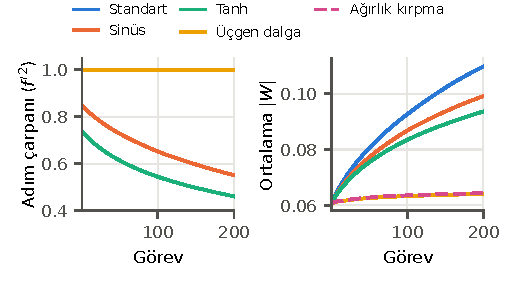
\includegraphics[width=\linewidth]{figures/sekil_mekanizma.pdf}
  \caption{Solda: ortalama adım çarpanı $\langle f'^2\rangle$. Sağda: ortalama ağırlık büyüklüğü. Ortalama ve
  \%95 aralığı; ölçümler beş görevde bir alınmıştır.}
  \label{fig:mekanizma}
\end{figure}

\begin{table}[t]
  \centering
  \caption{Mekanizma ölçütleri. $\langle f'^2\rangle$ ve doymuş oran akış sonundaki değerlerdir; oklar ilk
  pencereden son pencereye değişimi gösterir.}
  \label{tab:mekanizma}
  \setlength{\tabcolsep}{2.5pt}\footnotesize
  \resizebox{\linewidth}{!}{%
  \begin{tabular}{@{}lccccc@{}}
    \toprule
    Model & $\langle f'^2\rangle$ & Doymuş (\%) & Ort. $|W|$ & Adım normu & Etkin kerte\\
          &                       &             &            & (son/ilk)  & \\
    \midrule
    \satirlar{tablo_mekanizma.tex}
    \bottomrule
  \end{tabular}}
\end{table}

Şekil~\ref{fig:mekanizma} ve Tablo~\ref{tab:mekanizma} düzgün haritalardaki kaybın \eqref{eq:sonum} ile uyumlu
olduğunu göstermektedir. Sinüs ve tanh modellerinde ortalama ağırlık büyüklüğü akış boyunca artar (0,064'ten
0,098 ve 0,093'e); ağırlıklar sınıra yaklaştıkça ortalama adım çarpanı düzenli olarak düşer: sinüste 0,85'ten
0,56'ya, tanh'ta 0,74'ten 0,47'ye. Gerçekleşen ağırlık adımının normu da bununla tutarlı olarak ilk penceredeki
değerinin 0,85 ve 0,84 katına iner; standart ağda, üçgen dalgada ve ağırlık kırpmada bu oran birin biraz
üzerindedir. Bu ufukta tam doymuş ($|f'|<0{,}1$) parametrelerin oranı henüz düşüktür (sinüste \%4,3); kayıp, az
sayıda donmuş parametreden çok, bütün parametrelere yayılmış bir yavaşlamayla birlikte görülmektedir.

Üçgen dalgada adım çarpanı tanım gereği birdir ve ortalama ağırlık büyüklüğü akış boyunca neredeyse sabit kalır
(0,061'den 0,064'e); ağırlık kırpmada da aynı değerler ölçülmüştür. Son gizli katman temsilinin etkin kertesi
standart ağda 37'den 22'ye, sinüste 34'ten 21'e düşerken üçgen dalgada ve ağırlık kırpmada düşmez (33'ten 37 ve
38'e). Ölü birim oranı ise modeller arasında benzerdir (akış sonunda 0,12 ile 0,18 arası) ve gözlenen farkı
açıklamaz.

% ----------------------------------------------------------------------------------------------------
\section{Tartışma ve Sınırlılıklar}

Sonuçlar, bu deney düzeninde, ağırlıkların eleman bazında sınırlı olmasının tek başına yeterli olmadığını
düşündürmektedir: sinüs ve tanh modellerinde ağırlıklar kurgu gereği sınırlıdır, ancak plastisite kaybı sürer.
İşe yarayan iki yöntemin (üçgen dalga, ağırlık kırpma) ortak özelliği, sınırı sağlarken güncelleme büyüklüğünü
küçültmemeleridir. Düzgün haritaların standart ağa karşı küçük üstünlüğü, sınırın ağırlık büyümesini
yavaşlatmasıyla açıklanabilir; ancak aynı sınır adımları da küçültmektedir.

Üçgen dalga ile ağırlık kırpmanın ayırt edilememesi Bölüm~\ref{sec:yansima}'deki beklentiyle uyumludur: küçük adımlarda yansıma
ile izdüşüm arasındaki fark tek bir adımın büyüklüğünü aşmaz. Üçgen dalganın olası üstünlüğü başarımda değil,
kısıtın modelin bir parçası olmasındadır; bunun uygulamada bir yarar sağlayıp sağlamadığı bu çalışmada
sınanmamıştır.

Çalışmanın sınırlılıkları şunlardır. (i)~Tek bir veri kümesi ve küçük bir tam bağlı ağ kullanılmıştır.
(ii)~Akış kısadır (200 görev, görev başına 5.000 örnek); yavaş biriken bir bozulmanın değerlendirilmesi için
daha uzun akışlar gerekir. (iii)~Yalnızca stokastik gradyan inişi denenmiştir; uyarlamalı eniyileyicilerde adım
büyüklüğü aralığa göre büyük olabileceğinden sonuçlar farklı çıkabilir. (iv)~Sınır genişliği modeller arasında
farklıdır (her model için geliştirme akışında ayrı seçilmiştir); bu nedenle haritanın biçimi ile sınırın
genişliğinin etkileri bu deneyde tam olarak ayrıştırılmamıştır. (v)~Ağırlık kırpma beş tohumla çalıştırılmıştır.
(vi)~Sönümlemenin kaybın \emph{nedeni} olduğu burada doğrudan sınanmamıştır; ölçümler yalnızca bu açıklamayla
uyumludur. İleri yöndeki haritayı değiştirmeden yalnızca geri yöndeki türevi değiştiren bir müdahale deneyi ile
daha uzun akışlardaki deneyler sürmektedir.

% ----------------------------------------------------------------------------------------------------
\section{Sonuç}

Çevrim içi Permütasyonlu MNIST üzerinde 200 görevlik bir akışta, ağırlıkları düzgün bir harita ile sınırlamak
(sinüs, tanh) plastisite kaybını önlememiştir; bu modellerde ortalama adım çarpanı akış boyunca yaklaşık üçte bir
oranında düşmüştür. Türevi sıfıra yaklaşmayan üçgen dalga haritası kayıp göstermemiş ve ağırlık kırpma ile aynı
sonucu vermiştir. Bu ön bulgular, sınırlı bir ağırlık parametrizasyonunda sınırlılığın yanında güncelleme
büyüklüğünün korunmasının da önemli olduğuna işaret etmektedir. Bulguların daha uzun akışlarda, başka veri
kümelerinde ve başka eniyileyicilerde geçerli olup olmadığı ayrıca incelenmelidir.

\bibliographystyle{IEEEtran}
\bibliography{kaynaklar}

\end{document}
